\graphicspath{{./lab04/Images/}}


\maketitlepage{App Development}{in Android Studio}{Lab 4: Using Web APIs}
\maketocpage

\section{JSON}
JSON stands for JavaScript Object Notation. It is a human readable data format storing its data in key-value pairs. All its keys must be strings but the values can be strings, numerical values, other JSON objects, arrays, boolean values or even null. Keys and values are seperated by a colon while key-value pairs are seperated by a comma. A JSON object must be wrapped in curly brackets. An example of a JSON would be the following.
\begin{lstlisting}[style=A_JAVA]
{
	"name": "John",
	"age": 30,
	"courses": ["math", "programming"],
	"contact": {
		"phone": "9915311",
		"email": "john@mail.com"
	}
}
\end{lstlisting}
For those familiar with Python, this looks just like a literal dictionary although the keys and values are more restricted in JSON. The main purpose of JSON in this course is to get data from REST APIs but it has other purposes in general.

\subsection{JSONObject API}
The \texttt{JSONObject} class supports creating JSON objects from strings.
\begin{lstlisting}[style=A_Java]
String jsonString = "{" +
        "\"name\": \"John\"," + 
        "\"age\": 30," +
        "\"courses\": [\"math\", \"programming\"]," +
        "\"contact\": {\"phone\": \"9915311\", \"email\": \"john@mail.com\"}" +
"}";
try {
    JSONObject jsonObject = new JSONObject(jsonString);
} catch (JSONException e) {
    e.printStackTrace();
}
\end{lstlisting}
We can now parse this \texttt{JSONObject} but in order to do so, we must know the keys for any value we might want as well as the type of their corresponding value. We can parse the \texttt{JSONObject} above into Java types with the following code.
\begin{lstlisting}[style=A_Java]
try {
    JSONObject jsonObject = new JSONObject(jsonString);
    String name = jsonObject.getString("name");
    int age = jsonObject.getInt("age");
    JSONArray jsonArray = jsonObject.getJSONArray("courses");
    String course0 = jsonArray.getString(0);
    String course1 = jsonArray.getString(1);
    JSONObject nestedJsonObject = jsonObject.getJSONObject("contact");
    String phone = nestedJsonObject.getString("phone");
    String email = nestedJsonObject.getString("email");
} catch (JSONException e) {
    e.printStackTrace();
}
\end{lstlisting}
Another way to construct a JSON object is to create an initially empty object and add to it manually, like in the following code.
\begin{lstlisting}[style=A_Java]
try {
    JSONObject jsonObject = new JSONObject();
    jsonObject.put("key", "value");
    jsonObject.put("valid", false);
} catch (JSONException e) {
    e.printStackTrace();
}
\end{lstlisting}

\subsection{Gson API}
\texttt{Gson} is a library from Google that can convert Java objects into JSON and vice versa. Add the following to dependencies.
\begin{lstlisting}[style=A_txt]
compile group: 'com.google.code.gson', name: 'gson', version: '2.8.2'
\end{lstlisting}
Suppose we have the following class
\begin{lstlisting}[style=A_Java]
public class Person {
	String id;
	String name;
	int age;
	public Person(String id, String name, int age) {
		this.id = id;
		this.name = name;
		this.age = age;
	}
}
\end{lstlisting}
We can use \texttt{Gson} to construct a JSON object with an instance of this class where the keys are the name of its field and their values are the value of the instance. Having reference instance variable will result in a nested JSON object (given they are not String or arrays).
\begin{lstlisting}[style=A_Java]
Gson gson = new Gson();
Person person = new Person("A341#5_X", "Mortimer", 99);
String jsonPerson = gson.toJson(person);
// outcome: {"id": "A341#5_X", "name": "Mortimer", "age": 99}
\end{lstlisting}
To convert the other way around we can use reflection. Note that any missing field in the JSON object will be set to its default value and excessive keys will be ignored.
\begin{lstlisting}[style=A_Java]
Gson gson = new Gson();
String jsonString = "{\"id\": \"1A\", \"name\": \"Lisa\", \"age\": 45}"
Person person = gson.fromJson(jsonString, Person.class);
\end{lstlisting}
Like \texttt{JSONObject}, \texttt{gson} can also be used to add key-value pairs one by one to an intially empty JSON object.
\begin{lstlisting}[style=A_Java]
JsonObject jsonObject = new JsonObject();
jsonObject.addProperty("Key", "value");
\end{lstlisting}

\section{Calling web servers}
There are multiple ways to call a web server. It can be done using only Java standard library but that can be somewhat tedious having to build a client from scratch and use threading so we will use a library called \href{https://github.com/koush/ion}{ion}, an asynchronous networking and image loading library.\\

There are a lot of web servers out there and one will have to read their documentation to use them. Some provide means up getting data, uploading data, getting data based on input and so on. Others may requires keys or authentication. It will be your job to familiarize yourself with the webserver you want to use. The first example we will look at is a simple get request to the Chuck Norris API. Upon a click we get a joke and update some textview with it. To get a response for our API request, we can use the following given that we want the result as a string (other option include byte array or a \texttt{Gson} JSON object).
\begin{lstlisting}[style=A_Java]
Ion.with(/* your activity's context */)
        .load(/* url as string */)
        .asString() // if you want the results as String
        .setCallback(new FutureCallback<String>() {
            @Override
            public void onCompleted(Exception e, String result) {
                // when results are in
            }
});
\end{lstlisting}
There are various options available such as setting headers, body (for post requests), timeouts and if everything goes as expected, the exception parameter \texttt{e} should be \texttt{null}. If not, you should handle the exception appropriately (errors such as timeouts or invalid urls). The source code for the Chuck Norris example can be found \href{https://github.com/JonSteinn/AndroidDevelopment/tree/master/examples/lab4/chucknorris}{here} and a programming session making it \href{https://youtu.be/PS8CxRP2XjA}{here}.\\


\section{Creating a simple Web API (Optional)}
One approach to writing apps is to keep the logic stored on a webserver making Android do little more than update UI on events and serve as a client to the webserver. This way it is easy to extend your app to another platform. Now we will look at creating a very simple webserver with Flask. Feel free to adopt this to any other framework if you have prior knowledge of webservers or if you have some other preferences over using python. Note that the localhost of the emulator, your phone and your computer are not the same so having a webserver running on your localhost on your computer can not be accessed that way from the emulator or the phone. The emulator can us IP address \texttt{10.0.2.2} while you would probably have to deploy the server to use for your actual phone. In the provided example we create a very webserver that returns the square of a number. Note that you need \href{https://www.python.org/downloads/}{Python} and \href{http://flask.pocoo.org}{Flask} to run the server. The source code can be found \href{https://github.com/JonSteinn/AndroidDevelopment/tree/master/examples/lab4/squarenumber}{here}, the programming session \href{https://youtu.be/3i2AVI5w6VE}{here}, a silent video of python and flask setup \href{https://youtu.be/8Z4pielSO70}{here} and a guide how one can deploy the webserver \href{https://youtu.be/d15uchNJhak}{here}.

\begin{figure}[H]
\centering
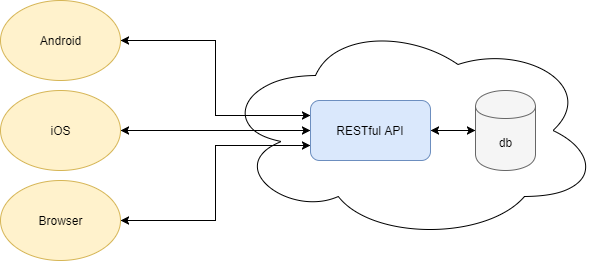
\includegraphics[scale=0.6]{web_api.png}
\caption{Shared logic for multiple platforms}
\label{fig:logshare}
\end{figure}

\section{Assignment}
Use the \href{https://developer.oxforddictionaries.com}{Oxford dictionaries API} to create an app where you can enter an english word and get its definition displayed. The app should also contain a choice between Spanish and German (or any two distinct non English languages) and display the word's meaning in that language. In order to do that you must get a key (there is a free one available) which you should add as header fields when making a request.

\begin{lstlisting}[style=A_Java]
Ion.with(this)
        .load(url)
        .addHeader("Accept", "application/json")
        .addHeader("app_id", "<someid>")
        .addHeader("app_key", "<somekey>")
        // and so on
\end{lstlisting}